\documentclass[../main.tex]{subfiles}
\begin{document}
\chapter{Higher Order Linear ODEs}
We will focus on 2nd order here, but many methods are also applicable to higher orders.
\section{Constant Coefficients}
The general form of a 2nd order linear ODE with constant coefficients is:
\begin{equation}
  \label{general2ndConst}
  \underbrace{a \deriv[2]{y}{x} + b \deriv{y}{x} + cy}_{\mathcal{D}y} = f(x)
\end{equation}
with $a, b, c$ constants.
Where $\mathcal{D}y$ is a linear differential operator, defined as:
\[
  \mathcal{D} \equiv a \deriv[2]{}{x} + b \deriv{}{x} + c
\]
\begin{definition}[Linear Operator]
  A differential operator, $\mathcal{D}$ is \textit{linear} if for any $y_1(x)$ and $y_2(x)$ and constants $\alpha$ and $\beta$:
  \[
    \mathcal{D}(\alpha y_1 + \beta y_2) = \alpha \mathcal{D}y_1 + \beta \mathcal{D}y_2
  \]
  This is also known as the \textit{principle of superposition}.
\end{definition}
We can exploit this property to solve \cref{general2ndConst}:
\begin{enumerate}
  \item Find complimentary functions (C.F.), $y_c$, that satisfy the corresponding homogeneous equation:
    \[
      a \deriv[2]{y_c}{x} + b \deriv{y_c}{x} + c y_c = 0
    \]
  \item Find \textbf{any} particular integral (P.I.), $y_p$ that satisfies the full equation.
  \item Then a solution of the full equation is then $y_c + y_p$ as:
    \[
      \mathcal{D}(y_c + y_p) = \underbrace{\mathcal{D}y_c}_{=0} + \mathcal{D}y_p = f(x)
    \]
    So it satisfies the full equation.
\end{enumerate}
A 2nd order ODE has \textbf{two} linearly independent complimentary functions, so the general solution to is:
\[
  y(x) = C_1 y_{c_1}(x) + C_2 y_{c_2}(x) + y_p(x)
\]
with $C_1, C_2$ constants.
\begin{definition}[Linear Dependance]
  A set of $n$ functions $\{f_i(x)\}$ is \textit{linearly dependant} if:
  \[
    \sum_{i=1}^{n} C_i f_i(x) = 0\ \forall x
  \]
  for $n$ constants, $C_i$, \textbf{not} all of which are $0$.
  Otherwise they are \textit{linearly independent}.
\end{definition}
\begin{remark}
  This is the same idea as linear dependence for vectors.
\end{remark}
Equivalently, if one or more of the functions $f_i(x)$  can be written as a linear combination of the others, they are linearly \textbf{dependant}.
\subsection{Complimentary Functions}
Recall that:
\[
  \deriv{}{x} e^{\lambda x} = \lambda e^{\lambda x} \text{ (Eigenfunction)}
\]
$e^{\lambda x}$ is also an eigenfunction of $\mathcal{D}$ because:
\begin{align*}
  \mathcal{D}(e^{\lambda x}) &= a \deriv[2]{}{x} e^{\lambda x} + b \deriv{}{x} e^{\lambda x} + c \\
                             &= \underbrace{(a\lambda^2 + b\lambda + c)}_{\text{eigenvalue}} e^{\lambda x}
\end{align*}
The complimentary functions of \cref{general2ndConst} satisfy $\mathcal{D}y_c = 0$, that is, they are eigenfunctions with eigenvalue $0$.
Thus:
\[
  y_c = A e^{\lambda x} \text{ with } \underbrace{a \lambda^2 + b\lambda + c = 0}_{\text{characteristic equation}}
\]
Since the characteristic equation of $\mathcal{D}$ is a 2nd degree polynomial it must have two roots $\lambda_1$ and $\lambda_2$.
\begin{proofcases}
  \begin{case}{$\lambda_1 \neq \lambda_2$}
    We then have two linearly independent complimentary functions:
    \[
      y_{c_1} \propto e^{\lambda_1 x}, y_{c_2} \propto e^{\lambda_2 x}
    \]
    So the most general complimentary function is a linear combination:
    \[
      y_c = C_1 y_{c_1}(x) + C_2 y_{c_2}(x)
    \]
    So $y_{c_1}$ and $y_{c_2}$ for a \textit{basis} for the space of solutions for the homogeneous equation.
    Note that if the roots are complex, we get oscillatory behaviour.
  \end{case}
  \begin{case}{$\lambda = \lambda_2$ -- Degenerate Case}
    So now we have only one linearly independent complimentary function of the form $e^{\lambda_1 x}$.
    See \cref{detuningExample} for how to deal with this case.
  \end{case}
\end{proofcases}
\begin{example}[Real, non-degenerate roots]
  \[
    \deriv[2]{y}{x} - 5\deriv{y}{x} + 6y = 0
  \]
  The characteristic equation is then:
  \[
    \lambda^2 - 5\lambda + 6 = 0 \implies \lambda_1 = 3, \lambda_2 = 2
  \]
  So the general complimentary function is:
  \[
    y_c(x) = A e^{3x} + B e^{2x}
  \]
  with $A, B$ constants.
\end{example}
\begin{example}[Complex, non-degenerate roots]
  \label{complexNonDegenerate}
  \[
    \deriv[2]{y}{x} + 4y = 0
  \]
  The characteristic equation is then:
  \[
    \lambda^2 + 4 = 0 \implies \lambda_1 = 2i, \lambda_2 = -2i
  \]
  So the general complimentary function is:
  \[
    y_c(x) = Ae^{2ix} + Be^{-2ix}
  \]
  Note that $e^{\pm2ix} = \cos(2x) \pm i \sin(2x)$ so:
  \begin{align*}
    y_c(x) &= (A + B)\cos(2x) + (A - B)i\sin(2x) \\
           &= \alpha \cos(2x) + \beta \sin(2x)
  \end{align*}
  Whether $\alpha, \beta$ are complex depends on the boundary conditions of the problem.
\end{example}
\begin{example}[Degenerate roots and ``detuning'']
  \label{detuningExample}
  \[
    \deriv[2]{y}{x} - 4\deriv{y}{x} + 4y = 0
  \]
  So the characteristic equation is:
  \[
    \lambda^2 - 4y + 4 = 0 \implies \lambda = 2
  \]
  Therefore we have degenerate roots and only one linearly independent complimentary function $e^{2x}$.

  \textbf{Detuning - }Remove the degeneracy by considering a slightly modified (\textit{detuned}) equation.
  \[
    \deriv[2]{y}{x} - 4 \deriv{y}{x} + (4 - \varepsilon^2)y = 0 \quad (\varepsilon \ll 1)
  \]
  So the characteristic equation is now:
  \[
    \lambda^2 - 4\lambda + (4 - \varepsilon^2) = 0 \implies \lambda = 2 \pm \varepsilon
  \]
  Which gives the complimentary function:
  \begin{align*}
    y_c(x) &= Ae^{(2 + \varepsilon)x} + Be^{(2 - \varepsilon)x} \\
           &=e^{2x}(Ae^{\varepsilon x} + Be^{-\varepsilon x}) \\
           &=e^{2x}[(A+B) + \varepsilon(A - B)x + O(A\varepsilon^2x^2) + O(B\varepsilon^2x^2)] \text{ (as $\varepsilon \to 0$)} \\
  \end{align*}
  Apply the initial conditions $y(0) = C$ and $y'(0) = D$ to both the original and detuned equations.
  This yields the equations:
  \begin{align*}
    &A + B = C \text{ and } 2C + \varepsilon(A - B) = D \\
    \implies& A = \frac{1}{2}\left(C + \frac{D - 2C}{\varepsilon}\right),\ B = \frac{1}{2}\left(C - \frac{D - 2C}{\varepsilon}\right)
  \end{align*}
  So $O(A) \text{ and } O(B) = O(\frac{1}{\varepsilon})$ as $\varepsilon \to 0$.
  Therefore $O(A\varepsilon^2x^2) \text{ and } O(B\varepsilon^2x^2) = O(\varepsilon x^2) \to 0$ as $\varepsilon \to0$.

  Now let:
  \[
    \alpha = A + B, \beta = \varepsilon(A - B)
  \]
  Both $\alpha$ and $\beta$ are $O(1)$ as they do not depend on $\varepsilon$ so are unchanged as $\varepsilon \to 0$.
  As we take $\varepsilon \to 0$, the detuned equation becomes the original equation, so the general solution of the original degenerate equation is:
  \[
    y = \alpha e^{2x} + \beta x e^{2x}
  \]
\end{example}
\begin{remark}[Note]
  In general, if $y_{c_1}$ is a degenerate complimentary function of a linear ODE with constant coefficients then $y_{c_2} = x y_{c_1}$ is a second linearly independent complimentary function.
\end{remark}
\section{Homogeneous Second Order ODEs with Non-constant Coefficients}
The general form of a homogeneous second order ODE with non-constant coefficients is:
\[
  y'' + p(x)y' + q(x)y = 0
\]
\subsection{Second Complimentary Function -- Reduction of order}
\label{reductionOrder}
The following method allows us to find a second solution, $y_2(x)$, given one solution, $y_1(x)$.

We try a solution of the form $y_2(x) = v(x)y_1(x)$.
Therefore:
\[
  y_2' = v'y_1 + vy_1' \text{ and } y_2'' = v''y_1 + 2v'y_1' + vy_1''
\]
If $y_2$ satisfies the original ODE then we require that:
\begin{align*}
  v''y_1 + v'(2y_1' + py_1) + v(\underbrace{y_1'' + py_1' + qy_1}_{0}) &= 0 \\
  v''y_1 + v'(2y_1' + py_1) &= 0
\end{align*}
We can then let $u = y'$ to reduce the order of the DE:
\[
  u'y_1 + u(2y_1' + py_1) = 0
\]
This is now a separable first order ODE for $u$.
\begin{align*}
  \frac{u'}{u} &= -\frac{2y_1'}{y_1} - p \\
  \implies \ln u &= -2 \ln y_1  - \int_{0}^{x} p(t) \d{t} + \ln A \\
  \implies u(x) &= \frac{A}{y^{2}_{1}}\exp\left[-\int_{0}^{x} p(t) \d{t}\right]
\end{align*}
We can then, in theory, integrate this expression for $u(x)$ to obtain $v(x)$.
\begin{example}
  Consider again the DE from \cref{detuningExample}:
  \[
    y'' - 4y' + 4y = 0
  \]
  So $p(x) = -4, q(x) = 4$.
  We know that one solution is $y_1(x) = e^{2x}$.
  \[
    \frac{u'}{u} = -\frac{4e^{2x}}{e^{2x}} - (-4) = 0
  \]
  So $u$ and therefore $v'$ are constants so:
  \[
    v(x) = Ax+B
  \]
  Therefore we have a second solution $y_2$ given by:
  \[
    y_2(x) = (Ax + B)e^{2x}
  \]
  The $Be^{2x}$ replicates $y_1$ so $xe^{2x}$ is a second linearly independent solution.
\end{example}
\subsection{Phase Space}
The general form of an $n$-th order linear ODE is:
\[
  y^{(n)} + p(x)y^{(n-1)} + \cdots + q(x)y = f(x)
\]
This means that $y^{(n)}$ is determined by $y^{(0)}, \ldots, y^{(n-1)}$.
When we differentiate the equation, we see that higher order derivatives can also be determined by $y^{(0)}, \ldots, y^{(n-1)}$.
This means that we can construct a Taylor series about $x_0$ if we specify $y^{(0)}(x_0), \ldots, y^{(n-1)}(x_0)$.

In other words, the \textit{state of the system} is fully specified at any $x$ by an $n$-dimensional \textit{solution vector}:
\[
  \vec{Y}(x) = \begin{pmatrix}
  y(x) \\
  y^{(1)}(x) \\
  \vdots \\
  y^{(n-1)}(x) \\
  \end{pmatrix}
\]
That is, given such a $\vec{Y}(x_0)$ at any fixed $x_0$, we can determine the Taylor series for the solution and use this to determine $y$ and all of its derivatives at any $x$.
\begin{remark}
  \begin{itemize}
    \item At any $x$, $\vec{Y}(x)$ defines a point in $n$-dimensional \textit{phase space}.
    \item As $x$ varies, $\vec{Y}(x)$ traces a trajectory through \textit{phase space}.
  \end{itemize}
\end{remark}
\begin{example}
  Consider again the DE from \cref{complexNonDegenerate}:
  \[
    y'' + 4y = 0
  \]
  We know that $y_1(x) = \cos 2x$ and $y_2(x) = \sin 2x$ so the solution vectors are:
  \[
    \vec{Y}_1 = \begin{pmatrix}
    y_1 \\
    y_1' \\
    \end{pmatrix} =
    \begin{pmatrix}
    \cos 2x \\
    -2\sin 2x \\
    \end{pmatrix},\
    \vec{Y}_2 = \begin{pmatrix}
    y_2 \\
    y_2 \\
    \end{pmatrix} =
    \begin{pmatrix}
    \sin 2x \\
    2 \cos 2x \\
    \end{pmatrix}
  \]
  So in 2D phase space, $\vec{Y}_1$ and $\vec{Y}_2$ lie on the same ellipse:
  \begin{center}
  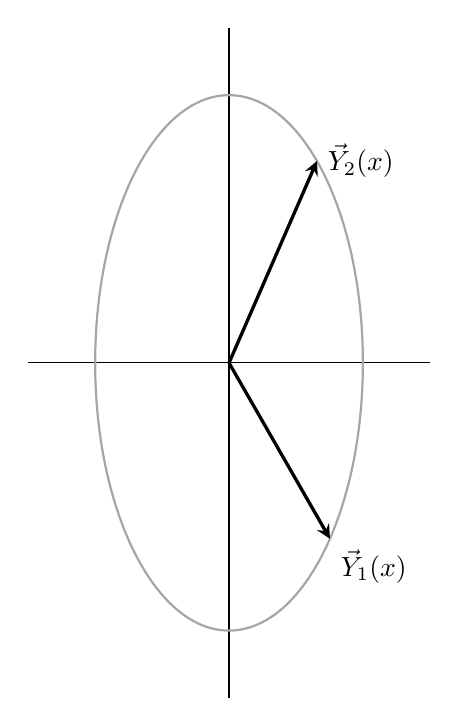
\begin{tikzpicture}[scale=1.7, >=stealth]
    \draw[-] (-1.5, 0) -- (1.5, 0);
    \draw[-] (0, -2.5) -- (0, 2.5);

    \draw[thick, gray!70] (0, 0) ellipse (1 and 2);

    \draw[->, very thick] (0, 0) -- (0.7539, -1.3139) node[below right] {$\vec{Y}_1(x)$};
    \draw[->, very thick] (0, 0) -- (0.6569, 1.5078) node[right] {$\vec{Y}_2(x)$};
  \end{tikzpicture}
  \end{center}
  $\vec{Y}_1$ and $\vec{Y}_2$ are linearly independent vectors.
  This means that they form a basis for the 2D phase space.
\end{example}
\section{Wronskian and Linear Dependence}
\label{wronskian}
Recall that a set of functions $\{y_i(x)\}$ are linearly dependant if:
\[
  \sum_{i=1}^{n} c_i y_i(x) = 0\ \forall x,\ c_i \text{ not all 0}
\]
Since this holds for all $x$ we can differentiate it $1, 2, \ldots, n-1$  times.
Therefore:
\[
  \sum_{i=1}^{n} c_i y^{(k)}_i(x) = 0\ \forall x, k = 1, \ldots, n-1
\]
This sum the $k$-th entry in the sum of all the solution vectors, so we have:
\[
  \sum_{i=1}^{n} c_i \vec{Y}_i(x) = 0\ \forall x
\]
So if $\{y_i\}$ is linearly dependant, then $\{\vec{Y}_i(x)\}$ are linearly dependant for all $x$.

We can form a \textit{fundamental matrix}, $\Psi(x)$, whose columns are the solution vectors:
\[
  \Psi(x) = \begin{pmatrix}
  \uparrow & \uparrow &  & \uparrow \\
  \vec{Y}_1 & \vec{Y}_2 & \cdots & \vec{Y}_n \\
  \downarrow & \downarrow &  & \downarrow \\
  \end{pmatrix}
\]
\begin{definition}[Wronskian]
  The \textit{Wronskian} of $n$ functions $\{y_i\}$ is defined to be the following determinant:
  \[
    W(x) =
    \begin{vmatrix}
      y_1 & y_2 & \cdots & y_n \\
      y_1' & y_2' & \cdots & y_n' \\
      \vdots & \vdots & \ddots & \vdots \\
      y^{(n-1)}_1 & y^{(n-1)}_2 & \cdots & y^{(n-1)}_n \\
    \end{vmatrix}
  \]
\end{definition}
\begin{remark}[Note]
  In this case, the Wronskian is the determinant of the fundamental matrix, that is:
  \[
    W(x) =
    \det(\Psi(x)) =
    \begin{vmatrix}
      \uparrow & \uparrow &  & \uparrow \\
      \vec{Y}_1 & \vec{Y}_2 & \cdots  & \vec{Y}_n \\
      \downarrow & \downarrow &  & \downarrow \\
    \end{vmatrix}
  \]
\end{remark}
Recall that if a matrix has linearly dependant columns then its determinant is 0.
Therefore we have:
\[
  \{y_i(x)\} \text{ is linearly \textbf{dependant}} \implies \{\vec{Y}_i(x)\} \text{ is linearly \textbf{dependant}} \implies W(x) = 0\ \forall x
\]
Taking the contrapositive, it follows that if $W(x) \neq 0$ for some $x$ then $\{y_i(x)\}$ are linearly \textbf{independent}.
\begin{remark}[Warning]
  $W(x) = 0\ \forall x$  does \textbf{not} necessarily imply that $\{y_i(x)\}$ are linearly dependant.
\end{remark}
\begin{example}
  Consider again the DE from \cref{complexNonDegenerate}:
  \[
    y'' + 4y = 0
  \]
  We can calculate the Wronskian using the solution vectors we found earlier:
  \[
    W(x) = \begin{vmatrix}
    y_1 & y_2 \\
    y_1' & y_2' \\
    \end{vmatrix} = \begin{vmatrix}
    \cos 2x & \sin2x \\
    -2\sin 2x & 2\cos 2x \\
    \end{vmatrix}
    = 2(\cos^2 2x + \sin^2 2x) = 2
  \]
  Since $W(x) \neq 0\ \forall x$, $y_1$ and $y_2$ are linearly independent.
\end{example}
\section{Abel's Theorem}
\begin{theorem}
  Given any two solutions of:
  \[
    y'' + p(x)y' + q(x)y = 0
  \]
  If $p(x)$ and $q(x)$ are continuous on an interval $I$, then either $W(x) = 0\ \forall x \in I$ or $W(x) \neq 0\ \forall x \in I$.
\end{theorem}
\begin{proof}
  \begin{align*}
    W(x) &= y_1 y_2' - y_2 y_1' \\
    W'(x) &= \cancel{y_1' y_2'} + y_1 y_2'' - \cancel{y_2' y_1'} - y_2 y_1'' \\
          &= y_1 y_2'' - y_2 y_1'' \\
          &= -y_1(py_2' + qy_2) + y_2(py_1' + qy_1) \\
          &= -p(x)(y_1 y_2' - y_2 y_1') \\
          &= -p(x)W(x)
  \end{align*}
  So we now have a separable ODE for $W(x)$, solving yields:
  \[
    W(x) = W(x_0)\underbrace{\exp\left[-\int_{x_0}^{x} p(u) \d{u}\right]}_{\neq0}
  \]
  This is known as \textit{Abel's identity}.
  The exponential is never 0 so:
  \begin{align*}
    W(x_0) = 0 &\implies W(x) = 0\ \forall x \\
    W(x_0) \neq 0 &\implies W(x) \neq 0\ \forall x
  \end{align*}
\end{proof}
\begin{remark}
  The geometric interpretation of this is the solution vectors are always collinear or never collinear as $x$ varies.
\end{remark}
\begin{remark}[Generalisation]
  Abel's theorem holds for solutions of $n$-th order linear homogeneous ODEs.
  There is also a generalisation of Abel's identity, see Example Sheet 3, Q7.
\end{remark}
\begin{corollary}
  If $p(x) = 0$ then $W(x)$ is a constant.
\end{corollary}
\begin{proof}
  Then $W'(x) = 0 \implies W(x) = C$.
\end{proof}
We can find $W(x)$ without knowing solutions to the ODE.
\begin{example}[Bessel's Equation]
  Consider the ODE:
  \begin{align*}
    x^2 y'' + xy' + (x^2 - n^2)y &= 0 \\
    y'' + \underbrace{\frac{1}{x}}_{p(x)}y' + \left(1 - \frac{n^2}{x^2}\right)y &= 0
  \end{align*}
  We can then apply Abel's identity so:
  \begin{align*}
    W(x) &= W(x_0)\exp\left[-\int_{x_0}^{x} \frac{\d{u}}{u}\right] \\
         &= W(x_0)\exp\left[-\ln\left(\frac{x}{x_0}\right)\right] \\
         &= \frac{W(x_0)x_0}{x}
  \end{align*}
\end{example}
\subsection{Finding Second Solutions}
Abel's identity can be used to find a second solution $y_2$ given a known solution $y_1$.
\[
  y_1 y_2' + y_2 y_1' = W(x_0)\exp\left[-\int_{x_0}^{x} p(u) \d{u}\right]
\]
Dividing by $y^{2}_{1}$ we have:
\[
  y_2' \frac{1}{y_1} + y_2 \frac{y_1'}{y^{2}_{1}} = \frac{W(x_0)}{y^{2}_{1}}\exp\left[-\int_{x_0}^{x} p(u) \d{u}\right]
\]
So provided we know $y_1$ this is a first order ODE for $y_2$:
\[
  \deriv{}{x}\left(\frac{y_2}{y_1}\right) = \frac{W(x_0)}{y^{2}_{1}}\exp\left[-\int_{x_0}^{x} p(u) \d{u}\right]
\]
This is the same result that we had using the reduction of order method in \cref{reductionOrder} as $W(x_0)$ is a constant.

\section{Linear Equidimensional ODEs}
\begin{definition}
  A linear second order ODE is \textit{equidimensional} if it has form:
  \begin{equation}
    \label{generalEquidimensional}
    ax^2 y'' + bx y' + cy = f(x)
  \end{equation}
  with $a, b, c$ constants.
\end{definition}
\begin{remark}[Note]
  These are called \textit{equidimensional} as quantities on the left hand side have consistent physical dimensions.
\end{remark}
\subsection{Scaling Property}
If it is homogeneous, then we have a scaling property of solutions.
\begin{proposition}
  If $g(x)$ is a solution of \cref{generalEquidimensional} with $f(x) = 0$, then so is $y = g(\alpha x)$ where $\alpha$ is a constant.
\end{proposition}
\begin{proof}
  \begin{align*}
    \deriv{}{x}(g(\alpha x)) &= \alpha g'(\alpha x) \\
    x \deriv{y}{x} &= (\alpha x)g'(\alpha x) \\
    x^2 \deriv[2]{y}{x} &= (\alpha x)^2 g''(\alpha x)
  \end{align*}
  Substituting back into \cref{generalEquidimensional} yields:
  \begin{align*}
    ax^2 \deriv[2]{y}{x} + bx \deriv{y}{x} + cy &= a (\alpha x)^2 g''(\alpha x) + b(\alpha x)g'(\alpha x) + cg(\alpha x) \\
                                                &= au^2 g''(u) + bu g'(u) + cg(u) \\
                                                &=0 \text{ as $g(u)$ is a solution}
  \end{align*}
  so $g(\alpha x)$ is also a solution.
\end{proof}

\subsection{Solving By Eigenfunctions}
\label{solvingByEigenfunctions}
Notice that:
\[
  x \deriv{}{x}(x^{k}) = k x^{k}
\]
so $x^{k}$ is an eigenfunction of $x \deriv{}{x}$ with eigenvalue $k$.
We will then look for a complimentary function of the form $y_c = x^{k}$.
\[
  x^{k}[ak(k - 1) + bk + c] = 0
\]
Since this is true for all $x$ we must have:
\[
  ak^2 + k(b - a) + c = 0
\]
In general this will have two roots $k_1, k_2$.
If $k_1 \neq k_2$ then the general complimentary function is:
\[
  y_c = Ax^{k_1} + Bx^{k_2}
\]
with $A, B$ constants.
\subsection{Solving By Substitution}
Substitute $z = \ln x$, so:
\[
  \deriv{y}{z} = \deriv{x}{z} \deriv{y}{x} = e^{z} \deriv{y}{x} = x \deriv{y}{x}
\]
\begin{align*}
  \deriv[2]{y}{z} &= e^{z} \deriv{y}{x} + e^{2z} \deriv[2]{y}{x} \\
                  &= x \deriv{y}{x} + x^2 \deriv[2]{y}{x}
\end{align*}
So \cref{generalEquidimensional} becomes:
\begin{align*}
  a\left(\deriv[2]{y}{z} - \deriv{y}{z}\right) + b \deriv{y}{z} + cy &= f(e^{z}) \\
  a \deriv[2]{y}{z} + (b - a)\deriv{y}{z} + cy &= f(e^{z})
\end{align*}
This is now a second order linear ODE with constant coefficients.
So $y_c \propto e^{\lambda z}$ and has characteristic equation:
\[
  a\lambda^2 + (b - a)\lambda + c = 0
\]
This will have the same solutions as the equation for $k_1, k_2$ from the eigenfunction method (\cref{solvingByEigenfunctions}).
In the non-degenerate case we have:
\begin{align*}
  y_c &= Ae^{k_1 z} + Be^{k_2 z} \\
      &= Ax^{k_1} + Bx^{k_2}
\end{align*}
We also know from \cref{detuningExample} that in the degenerate case we have:
\begin{align*}
  y_c &= Ae^{kz} + Bze^{kz} \\
      &= Ax^{k} + B(\ln x)x^{k}
\end{align*}

\section{Inhomogeneous (Forced) 2nd Order ODEs}
This section covers methods to find particular integrals.
\subsection{Constant Coefficients}
Recall that these have general form:
\[
  a \deriv[2]{y}{x} + b \deriv{y}{x} + cy = f(x)
\]
After we have found the complimentary function we need to determine a single particular integral.
It is helpful to know what kind of particular integrals are likely to work for different types of forcing function $f(x)$.
In general, this is the most ``general'' form of the type of function $f$ is, for example:
\begin{center}
\begin{tabular}{c|c}
\label{PITable}
$f(x)$ & Try particular integral of form \\
\hline
$e^{mx}$ & $Ae^{mx}$ \\
$\sin kx$ or $\cos kx$ & $A \sin kx + B \cos kx$ \\
Polynomial $p_n(x)$ & Polynomial $q_n (x) = a_nx^{n} + a_{n - 1}x^{n-1} + \cdots + a_1 x + a_0$ \\
\end{tabular}
\end{center}
We can then determine the constants in these particular integrals by substituting into the ODE.
Since it is a linear ODE, we can also superpose terms to try and find a particular integral.

\begin{example}
  Consider the ODE:
  \[
    y'' - 5y' + 6y = 2x + e^{4x}
  \]

  Try a particular integral $y_p = \underbrace{Ax + B}_{\text{for }2x} + \underbrace{Ce^{4x}}_{\text{for }e^{4x}}$.
  \begin{align*}
    y_p' &= A + 4Ce^{4x} \\
    y_p'' &= 16Ce^{4x}
  \end{align*}
  Substituting back into the DE and comparing coefficients:
  \[
    (\underbrace{16C - 20C + 6C}_{=1})e^{4x} + (\underbrace{6A}_{=2})x + (\underbrace{-5A + 6B}_{=0}) = 2x + e^{4x}
  \]
  Therefore we have $2C = 1 \implies C = \frac{1}{2}$, $6A = 2 \implies A = \frac{1}{3}$, $6B = \frac{5}{3} \implies B = \frac{5}{18}$.
  So:
  \[
    y_p = \frac{1}{3}x + \frac{5}{18} + \frac{1}{2}e^{4x}
  \]
  The complimentary function is:
  \[
    y_c = \alpha e^{2x} + \beta e^{3x}
  \]
  Therefore, the general solution is:
  \[
    y = \alpha e^{2x} + \beta e^{3x} + \frac{1}{2}e^{4x} + \frac{1}{3}x + \frac{5}{18}
  \]
  for constants $\alpha, \beta$.
\end{example}
\subsubsection{Resonance}
What if the forcing term, $f(x)$, involves a term that is in a complimentary function?
We can solve this using detuning again.
\begin{example}
  Consider the ODE:
  \[
    \ddot{y} + \omega_0^2 y = \sin(\omega_0 t)
  \]
  The homogeneous form of this is simple harmonic motion with angular frequency $\omega_0$.
  However, we have a forcing term at a \textit{natural frequency} $\omega_0$.
  We say that the oscillator is driven \textit{resonantly} because:
  \[
    y_c(t) = A\sin(\omega_0 t) + B\cos(\omega_0 t)
  \]
  so the oscillator is driven at a forcing frequency equal to the natural frequency.
  Consider the detuned equation:
  \[
    \ddot{y} + \omega^{2}_{0} y = \sin(\omega t)
  \]
  for some $\omega \neq \omega_0$.

  Try a particular integral $y_p(t) = C\sin(\omega t) + D \cos(\omega t)$:
  \begin{align*}
    \dot{y_p} &= C\omega\cos(\omega t) - D\omega\sin(\omega t) \\
    \ddot{y_p} &= -C\omega^2\sin(\omega t) - D\omega^2\cos(\omega t)
  \end{align*}
  Therefore:
  \[
    (C\omega^{2}_{0} - C\omega^2)\sin(\omega t) + (D\omega^{2}_{0} - D\omega)\cos(\omega t) = \sin(\omega t)
  \]
  So $D = 0$ and:
  \[
    (\omega^{2}_{0} - \omega^2)C = 1 \implies C = \frac{1}{\omega^{2}_{0} - \omega^2}
  \]
  However, notice that the limit as $\omega \to \omega_0$ does not exist.

  We can try adding in a complimentary function to regularise the limit.
  \[
    y_p(t) = \frac{1}{\omega^{2}_{0} - \omega^2}(\sin(\omega t) - \underbrace{\sin(\omega_0 t)}_{C.F.})
  \]
  Since we have just added a complimentary function, this still satisfies the detuned equation.
  We can now try to evaluate this indeterminate limit using L'H\^opitals rule, \cref{LHopitals}:
  \[
    \lim_{\omega \to \omega_0} y_p(t) = \lim_{\omega \to \omega_0} \left[\frac{t\cos(\omega t)}{-2\omega}\right] =-\frac{t}{2\omega_0}\cos(\omega_0 t)
  \]
  Therefore the particular integral of the original equation is:
  \[
    y_p(t) = -\frac{t}{2 \omega_0}\cos(\omega_0 t)
  \]
  Notice that the amplitude of this solution grows with $t$, this is referred to as \textit{resonance}.
\end{example}
In general, if the forcing term is a linear combination of complimentary functions, the particular integral is of the form:
\[
  y_p(t) = t \times (\text{Non-resonant P.I})
\]
We can obtain the non-resonant particular integral from the earlier table in \cref{PITable}.

\begin{remark}[Note]
  If the homogeneous equation is degenerate, we may need to try:
  \[
    y_p(t) = t^2 \times (\text{Non-resonant P.I.})
  \]
  as the complimentary function will already have a term with a factor of $t$.
\end{remark}
\subsubsection{Resonances in Equidimensional ODEs}
Consider:
\[
  ax^2y'' + bxy' + cy = f(x)
\]
We know that the general complimentary function is:
\[
  y_c = Ax^{k_1} + Bx^{k_2}
\]
provided we are in the non-degenerate case ($k_1 \neq k_2$).

If $f(x) \propto x^{m}$, then we should try a particular integral of the form $Cx^{m}$  for $m \neq k_1$ and $m \neq k_2$.
In the resonant case, $f(x) \propto x^{k_1} \text{ or }x^{k_2}$, then the particular integral is:
\[
  y_p \propto (\ln x) x^{k_1}
\]
This follows from transforming by $z = \ln x$.
The particular integral is $y_p = ze^{k_1 z}$ in the case of constant coefficients.
This is then $(\ln x)x^{k_1}$ after substituting back in with $x$.
\begin{remark}[Note]
  If the homogeneous equation is degenerate $(k_1 = k_2)$, we may need to try:
  \[
    y_p = (\ln x)^2 x^{k_1}
  \]
\end{remark}
\subsection{Variation of Parameters}
Variation of parameters is a systematic method to find a particular integral given two linearly independent complimentary functions.

Consider the general form of a 2nd order linear ODE with non-constant coefficients:
\[
  y'' + p(x)y' + q(x)y = f(x)
\]
with linearly independent complimentary functions $y_1$ and $y_2$.
Since we know that $y_1$ and $y_2$ are linearly independent, the solution vectors $\vec{Y}_1(x)$ and $\vec{Y}_2(x)$ are linearly independent for all $x$ so we can use them as a basis for phase space at any $x$.

Because they form a basis, we can write the solution vector for the particular integral, $\vec{Y}_p$, as a linear combination of $\vec{Y}_1$ and $\vec{Y}_2$ where the coefficients are functions of $x$:
\[
  \vec{Y}_p(x) = u(x)\vec{Y}_1(x) + v(x)\vec{Y}_2(x)
\]
We can from equations using the components of this to make it easier to solve:
\begin{align*}
  \text{First Component: }&y_p(x) = u(x)y_1(x) + v(x)y_2(x) \\
  \text{Second Component: }&y_p(x)' = u(x)y_1'(x) + v(x)y_2'(x)
\end{align*}
Start by taking the derivative of the second component:
\[
  y_p'' = u y_1'' + u'y_1' + vy_2'' + v'y_2'
\]
from the original ODE we have:
\begin{align*}
  f(x) &= y_p'' + py_p' + qy_p \\
       &= uy_1'' + u' y_1' + vy_2'' + v'y_2' + p(x)[uy_1' + vy_2'] + q(x)[uy_1 + vy_2] \\
       &= u[\underbrace{y_1'' + p(x)y_1' + q(x)y_1}_{=0}] + v[\underbrace{y_2'' + p(x)y_2' + q(x)y_2}_{=0}] + u'y_1' + v'y_2' \\
       &= u'y_1' + v'y_2'
\end{align*}
since $y_1$ and $y_2$ are complimentary functions.

The second component must be consistent with the derivative of the first component, therefore:
\begin{align*}
  u'y_1 + \cancel{uy_1'} + v'y_2 + \cancel{vy_2'} &= \cancel{uy_1'} + \cancel{vy_2'} \\
  u' y_1 + v' y_2 &= 0
\end{align*}
We can then combine these two equations into a matrix equation:
\begin{align*}
  \begin{pmatrix}
  y_1 & y_2 \\
  y_1' & y_2' \\
  \end{pmatrix}
  \begin{pmatrix}
  u' \\
  v' \\
  \end{pmatrix}&=
  \begin{pmatrix}
  0 \\
  f \\
  \end{pmatrix}\\\implies
  \begin{pmatrix}
  u' \\
  v' \\
  \end{pmatrix}&=
  \frac{1}{W}
  \begin{pmatrix}
  y_2' & -y_2 \\
  -y_1' & y_1 \\
  \end{pmatrix}
  \begin{pmatrix}
  0 \\
  f \\
  \end{pmatrix}
\end{align*}
Where $W(x) = y_1 y_2' - y_2 y_1'$ is the Wronskian, \cref{wronskian}.
Therefore:
\[
  u' = - \frac{y_2}{W}f,\ v' = \frac{y_1}{W}f
\]
We can then integrate to yield:
\[
  u = \int^{x} \frac{y_1(t)f(t)}{W(t)} \d{t},\ v = \int^{x} \frac{y_2(t)f(t)}{W(t)} \d{t}
\]
Substituting back into the equation from the first component yields:
\[
  y_p(x) = y_2(x)\int^{x} \frac{y_1(t)f(t)}{W(t)} \d{t} - y_1(x) \int^{x} \frac{y_2(t)f(t)}{W(t)} \d{t}
\]
Note that changing the lower limit/including an integration constant is unnecessary as it only adds multiples of the complimentary functions so the particular integral will still satisfy the original ODE regardless.
\end{document}
